\documentclass[a4paper,10pt]{article}
\usepackage[utf8]{vietnam}
\usepackage{float}
\usepackage{hyperref}
\usepackage{minted}
\usepackage{graphicx}
\usepackage[margin=2cm]{geometry}
\newcommand{\mnt}[1]{\inputminted[frame=single, linenos=true, tabsize=4]{c++}{#1}}
\title{\textbf{ĐỒ ÁN I }\\Các thuật toán trên đồ thị}
\author{Phạm Văn Thông}
\date{Ngày 22 tháng 5 năm 2015}
\begin{document}

\section{Đồ thị}
\subsection{Một số khái niệm cơ bản về đồ thị}
\subsubsection{Khái niệm đồ thị}
Đồ thị là một cấu trúc rời rạc gồm các đỉnh và các cạnh nối với các đỉnh đó. Được mô tả hình thức: $G = (V, E)$. Trong đó, V là tập các \textbf{đỉnh}, E gọi là tập các \textbf{cạnh}. Có thể coi E là tập các cặp $(u, v)$ với u và v là hai đỉnh của V.

Một số hình ảnh của đồ thị:
\begin{figure}[h!]
  \centering
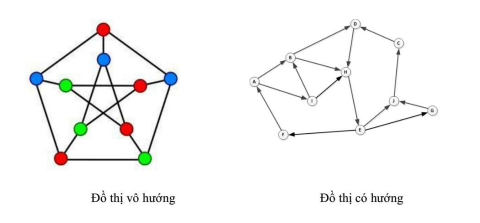
\includegraphics[scale=0.5]{images/pic1.png}
\end{figure}

\subsubsection{Các khái niệm cơ bản}
Có thể phân loại đồ thị theo đặc tính và số lượng tập cạnh E. Cho đồ thị $G = (V, E)$, ta có một số khái niệm sau:
\begin{description}
\item[Đơn đồ thị ] G được gọi là đơn đồ thị nếu giữa hai đỉnh u, v của V có nhiều nhất là một cạnh nối trong E nối từ u tới v.
\item[Đa đồ thị] G được gọi là đa đồ thị nếu giữa hai đỉnh u, v của V có thể có thể có nhiều hơn 1 cạnh trong E nối từ u tới v.
\item[Đồ thị vô hướng] G được gọi là đồ thị vô hướng nếu các cạnh trong E không định hướng, tức là cạnh nối hai đỉnh u, v bất kì cũng là cạnh nối hai đỉnh v, u. Hay nói cách khác, tập E gồm các cặp (u, v) không có tính thứ tự $(u, v) \equiv (v, u)$
\item[Đồ thị có hướng] G được gọi là đồ thị có hướng nếu các cạnh trong E là có định hướng, có thể có cạnh nối từ đỉnh u tới đỉnh v nhưng chưa chắc đã có chạn nối từ đỉnh v tới đỉnh u. Hay nói cách khác, tập E gồm các cặp (u, v) có tính thứ tự: $(u, v) \neq (v, u)$
\end{description}

\textbf{Ví dụ:}
\begin{figure}[h!]
  \centering
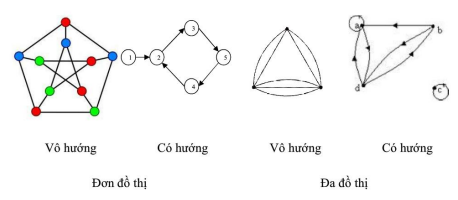
\includegraphics[scale=0.5]{images/pic2.png}
\end{figure}


\subsubsection{Cạnh liên thuộc, đỉnh kề, bậc}
Đối với \emph{đồ thị vô hướng } $G = (V, E)$, xét một cạnh $e \in E$, nếu $e = (u, v)$ thì ta nói hai đỉnh u và v là \textbf{kề nhau} (adjacent) và cạnh e này \textbf{liên thuộc} (incident) với đỉnh u và đỉnh v.

Với một đỉnh v trong đồ thị, ta định nghĩa \textbf{bậc} (degree) của v, kí hiệu deg(v) là số cạnh liên thuộc với v. Dễ thấy rằng trên đơn dồ thị thì số cạnh liên thuộc với v cũng là số đỉnh kề với v.

Đối với \emph{đồ thị có hướng} $G = (V, E)$. Xét một cung $e \in E$, nếu $e = (u, v)$ thì ta nói \textbf{u nối tới v} và \textbf{v nối từ u}, cung e là \textbf{đi ra khỏi đỉnh u và đi vào đỉnh v}. Đỉnh u khi đó được gọi là đỉnh đầu, đỉnh v được gọi là đỉnh cuối của cung e.

Với mỗi đỉnh v trong \emph{đồ thị có hướng}, ta định nghĩa: \textbf{Bán bậc ra } của v là số cung đi ra khỏi nó, \textbf{bán bậc vào } là số cung đi vào đỉnh đó.

\textbf{Đường đi:} Một đường đi độ dài k từ đỉnh u đến đỉnh v là dãy $(u=x_0, x_1, x_2, ... , x_k=v)$ thỏa mãn $(x_i, x_{i+1}) \in E$ với $\forall i$: $(0 \leq i \leq k)$. Đỉnh u gọi là đỉnh xuất phát, v gọi là đỉnh kết thúc đường đi. Đường đi không có cạnh nào đi qua hơn 1 lần được gọi là \textbf{đường đi đơn}.

\textbf{Chu trình:}Đường đi có đỉnh xuất phát trùng với đỉnh kết thúc gọi là \textbf{chu trình}, tương tự ta có khái niệm \textbf{chu trình đơn}.

\subsection{Bài toán tìm kiếm trên đồ thị}
\subsubsection{Phát biểu bài toán}
Cho đồ thị $G = (V, E)$ và s và t là hai đỉnh của đồ thị.
\emph{Yêu cầu: } Hãy chỉ ra một đường đi từ s đến t (nếu có).

\emph{Ví dụ: Xét một đồ thị vô hướng và một đồ thị có hướng dưới đây:}
\begin{figure}[h!]
  \centering
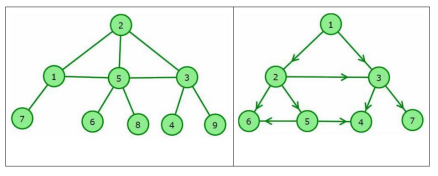
\includegraphics[scale=0.5]{images/pic3.png}
\end{figure}

Trên cả hai đồ thị, $(1, 2, 3, 4)$ là đường đi đơn độ dài 3 từ đỉnh 1 tới đỉnh 4. Bởi $1, 2)$, $(2, 3)$, $(3, 4)$ đều là các cạnh (hay cung).

Làm sao để duyệt tất cả các đỉnh có thể đến được từ một đỉnh xuất phát nào đó? Vấn đề này đưa về một bài toán liệt kê mà yêu cầu của nó là không được bỏ sót hay lặp lại bất kì đỉnh nào. Vì vậy, cần phải xây dựng những thuật toán cho phép duyệt một cách hệ thống các đỉnh, những thuật toán như vậy gọi là những thuật toán tìm kiếm trên đồ thị. Trong lý thuyết đồ thị, người ta quan tâm đến hai thuật toán cơ bản nhất: thuật toán tìm kiếm theo chiều sâu và thuật toán tìm kiếm theo chiều rộng.

\subsubsection{Thuật toán DFS}
Tư tưởng của thuật toán được trình bày như sau: Bắt đầu từ s, mọi đỉnh u kề với s tất nhiên sẽ đến được từ s. Với mỗi đỉnh u đó, những đỉnh v kề với u cũng đến được từ s... Ý tưởng đó gợi ý cho ta viết một thủ tục đệ quy DFS(u) mô tả việc duyệt từ đỉnh u bằng cách thông báo thăm đỉnh u và tiếp tục quá trình duyệt DFS(v) với v là một đỉnh chưa thăm kề với u. Để quá trình duyệt không lặp lại bất kì đỉnh nào, ta dùng kĩ thuật đánh dấu, khi thăm một đỉnh, ta sẽ đánh dấu đỉnh đó để các bước duyệt đệ quy tiếp theo không thăm lại đỉnh đó nữa.

Vấn đề còn lại: để in ra được đường đi từ đỉnh xuất phát s, trong quá trình duyệt DFS(u), trước khi gọi đệ quy DFS(v) với v là một đỉnh kề với u mà chưa đánh dấu, ta lưu lại \textbf{vết} đường đi từ u tới v bằng cách đặt \textsf{trace[v] = u}, tức là \textsf{trace[v]} là đỉnh liền trước v trong đường đi từ s tới v. Khi quá trình tìm kiếm theo chiều sâu kết thúc, đường đi từ S tới F sẽ là:
$$t \leftarrow trace[t] \leftarrow \ldots \leftarrow trace[u_1] \leftarrow \ldots \leftarrow trace[s] \leftarrow s$$

Truy ngược đường đi này sẽ cho ta hành trình đi từ s đến t. Có thể mô tả thủ tục DFS dưới dạng giả mã như sau:


\begin{minted}[frame=single, linenos=true]{C}
void DFS(vertice u)
{
  < 1. Thong bao da toi duoc u >;
  < 2. Danh dau u la da tham >;
  foreach (v ke voi u)
  if (v chua duoc tham)
  {
    trace[v] = u; //Truy vet duoc di
    DFS(v); //Goi de quy bat dau voi v
  }
}

void DFSPath()
{
  < Input: do thi G, s, t >;
  < Khoi tao: Tat ca cac dinh deu chua bi danh dau >;

  DFS(s);

  if (v chua bi danh dau)
     <Thong bao khong co duoc di tu s->t>;
  else
     <Dua vao trace tim duong di tu s->t>;
}
\end{minted}

\subsubsection{Thuật toán tìm kiếm theo chiều rộng BFS}
Ý tưởng của phương pháp này là \emph{lập lịch} duyệt các đỉnh. Khi thăm một đỉnh ta sẽ lên lịch thăm tất cả các đỉnh kề nó sao cho thứ tự duyệt là ưu tiên chiều rộng (đỉnh nào gần s hơn sẽ được duyệt trước).

\emph{Ví dụ: }
\begin{quotation}
  Bắt đầu ta thăm đỉnh s. Quá trình thăm s sẽ lên lịch duyệt những đỉnh $(u_1, u_2, \ldots , u_p)$ kề với s (những đỉnh gần s nhất). Tiếp theo sẽ thăm đỉnh $u_1$, khi thăm $u_1$ sẽ lại lên lịch duyệt những đỉnh $(v1, v2, \ldots , v_q)$ kề với $u_1$. Nhưng rõ ràng các đỉnh này xa s hơn những đỉnh u nên chúng chỉ được duyệt đến khi tất cả những đỉnh u đã duyệt xong, tức là thứ tự duyệt đỉnh sau khi đã thăm $u_1$ sẽ là: $(u_2, u_3, \ldots , u_p, v1, v2, \ldots , v_q )$. Do việc lập lịch như mô tả ở trnê nên cần phải xếp hàng cho các đỉnh đã lên lịch theo đúng thứ tự. Khi thêm đỉnh nào đó, ta sẽ thêm vào cuối hàng. Chính vì nguyên tắc đó nên danh sách chứa những đỉnh đang chờ sẽ được tổ chức dưới dạng hàng đợi - \emph{queue}.
\end{quotation}
Ta sẽ xây dựng giải thuật như sau:
\begin{minted}[frame=single, linenos=true]{C++}

void BFS(vertice v)
{
  //Khoi tao
  free[s] = true;
  free[v] = false; //v in V, v != s
  queue.push(v); //queue chi chua v

  while (!queue.empty())
  {
    u = queue.pop();
    free[u] = false;
    foreach(v ke voi u)
    if (free[v] == true)
    {
      free[v] = false;
      trace[v] = u;
      queue.push(v);
    }
    //Cac dinh ke u da duoc ghe tham
}

void BFSPath()
{
  < Input: do thi G, s, t >;
  < Khoi tao: Tat ca cac dinh deu chua bi danh dau >;

  BFS(s);

  if (v chua bi danh dau)
     <Thong bao khong co duoc di tu s->t>;
  else
     <Dua vao trace tim duong di tu s->t>;
}
\end{minted}

\subsubsection{Độ phức tạp của thuật toán DFS và BFS}
Quá trình tìm kiếm trên đồ thị bắt đầu từ một đỉnh có thể thăm các đỉnh còn lại, khi đó cách biểu diễn đồ thị có ảnh hưởng lớn tới chi phí về thời gian thực hiện giải thuật.

Trong trường hợp ta biểu diễn đồ thị bằng danh sách kề, cả hai thuật toán BFS và DFS đều có độ phức tạp tính toán là $O(n+m) = O(max(n, m))$. Đây là cách cài đặt tốt nhất. Nếu ta biểu diễn đồ thị bằng ma trận kề thì độ phức tạp tính toán trong trường hợp này là $O(n + n^2) = O(n^2)$. Nếu ta biểu diễn đồ thị bằng danh sách cạnh, thao tác duyệt những đỉnh kề với đỉnh u sẽ dẫn tới phải duyệt qua toàn bộ danh sách cạnh, đây là cài đặt tồi nhất, nó có độ phức tạp tính toán là $O(n.m)$.

\subsection{Bài toán tìm đường đi ngắn nhất trên đồ thị có trọng số}
\subsubsection{Phát biểu bài toán}
Bài toán được phát biểu dưới dạng tổng quá như sau: Cho đồ thị $G = (V, E)$ là đồ thị không có chu trình âm. Hãy tìm một đường đi ngắn nhất (tổng trọng số qua các đỉnh trên đường đi là bé nhất ) từ đỉnh xuất phát $s \in V$ đến đỉnh  đích $t \in V$. Nếu như đồ thị có chu trình âm thì khoảng cách giữa một số cặp đỉnh nào đó có thể không xác định vì bằng cách đi vòng theo chu trình này một số lần đủ lớn, ta có thể chi ra đường đi giữa hai đỉnh nào đó trong chu trình nayf nhỏ hơn bất kì một số cho trước nào. Trong trường hợp như vậy có thể đặt vấn đề tìm đường đi cơ bản (đường đi không có đỉnh lặp lại) ngắn nhất. Vấn đề đó là một bài toán hết sức phức tạp mà ta không bàn tới ở đây.

Dưới đây trình bày hai thuật toán để giải bài toán này là thuật toán Bellman-Ford và thuật toán Dijkstra.

\subsubsection{Giới thiệu thuật toán Bellman-Ford}
Thuật toán Bellman-Ford có thể phát biểu rất đơn giản:

\begin{quote}
  Với đỉnh xuất phát S, gọi d(v) là khoảng cách từ S tới v. Ban đầu d(S) được gán bằng 0, còn các d(v) với $v \neq S$ được khởi gán bằng $+\infty$

Sau đó, ta tối ưu hóa dần các d(v) như sau:
\begin{quotation}
  Xét mọi cặp đỉnh u, v của đồ thị, nếu có một cặp đỉnh u, v mà $d(v) > d(u) + c(u, v)$ thì ta đặt lại $d(v) = d(u) + c(u, v)$. Tức là độ dài đường đi từ S tới v lại lớn hơn tổng độ dài đường đi từ S tới u cộng với chi phí đi từ u tới v thì ta sẽ hủy bỏ đường đi từ S tới v đang có và coi đường đi từ S tới v chính là đường đi từ S tới u, sau đó đi tiếp từ u tới v.

Chú ý rằng ta đặt $c[u, v] = +\infty$ nếu (u, v) không là cung. Thuật toán sẽ kết thúc khi không thể tối ưu thêm bất kì một nhãn d[v] nào nữa.
\end{quotation}

\paragraph{Tính dừng của thuật toán}
\begin{description}
\item[Tại bước lặp 0] Bước khởi tạo $d(S) = 0; d(v) = +\infty$ với $v \neq S$ thì dãy d(v) chính là độ dài đường đi ngắn nhất từ S tới v qua không quá 0 cạnh.
\item[Tại bước lặp thứ i] d(v) bằng độ dài ngắn nhất từ S tới v qua không quá i cạnh, do tính chất đường đi từ S tới v qua không quá $i+1$ cạnh sẽ phải thành lập bằng cách lấy một đường đi từ S tới một đỉnh u nào đó qua không quá i cạnh rồi đi tiếp tới v bằng cung (u, v) nên độ dài đường đi ngắn nhất từ S tới v qua không quá $i+1$ cạnh sẽ được tính bằng giá trị nhỏ nhất trong các giá trị (Nguyên lý tối ưu Bellman):
  \begin{itemize}
  \item Độ dài đường đi ngắn nhất từ S tới v qua không quá i cạnh
  \item Độ dài đường đi ngắn nhất từ S tới u qua không quá i cạnh cộng với trọng số cạnh (u, v) $(\forall u)$
  \end{itemize}
nên sau bước lặp tối ưu các d(v) bằng công thức $d(v)_{bước i+1} = min(d(v)_{bước i}, d(u)_{bước i} + c(u, v))$ thì các d(v) sẽ bằng độ dài đường đi ngắn nhất từ S tới v qua không quá $i+1$ cạnh.
\item[Sau bước lặp tối ưu hóa thứ n-1] Ta có d(v) là độ dài đường đi ngắn nhất từ S tới v qua không quá n-1 cạnh. Vì đồ thị không có chu trình âm nên sẽ có một đường đi ngắn nhất từ S tới v là đường đi cơ bản (qua không quá n-1 cạnh). Tức là d(v) sẽ là độ dài đường đi ngắn nhất từ S tới v.
\end{description}

\textbf{Vậy thì số bước lặp tối ưu hóa sẽ không quá n-1 bước.}

Nếu mỗi bước ta mô tả dưới dạng:
\begin{minted}[frame=single]{C}
for (u=0; u<n; u++)
    for (v=0; v<n; v++)
        if (d[v] > d[u] + c[u][v])
            d[v] = d[u] + c[u][v];
\end{minted}
Do sự tối ưu bắc cầu (dùng d(u) tối ưu d(v) rồi lại có thể dùng d(v) tối ưu d(w) nữa ...) nên chỉ làm tốc độ tối ưu nhan d(v) tăng lên chứ không thể giảm đi được.

\end{quote}

\subsubsection{Giới thiệu thuật toán Dijkstra}
Thuật toán Dijkstra (E.Dijkstra - 1959) có thể mô tả như sau:
\begin{description}
\item[Bước 1: Khởi tạo ] Với đỉnh $v \in V$, gọi nhãn d[v] là độ dài đường đi ngắn nhất từ s tới v. Ta sẽ tính các d[v]. Ban đầu d[v] được khởi gán bằng c[s][v]. Nhãn của mỗi đỉnh có hai trạng thái tự do hay cố định, nhãn tự do nghĩa là có thể tối ưu hơn được nữa, và nhãn cố định tức là d[v] đã là độ dài đường đi ngắn nhất từ s tới v nên không thể tối ưu thêm. Để làm điều này ta có thể sử dụng kĩ thuật đánh dấu $free[v] = true$ hay $false$ tùy theo d[v] tự do hay cố định. Ban đầu các nhãn đều tự do.
\item[Bước 2: Lặp]

  \begin{itemize}
  \item Cố định nhãn: Chọn trong các đỉnh có nhãn tự do, lấy ra đỉnh u là đỉnh có d[u] nhỏ nhất và cố định nhãn đỉnh u.
  \item Sửa nhãn: Dùng đỉnh u xét tất cả những đỉnh v và sửa lại các d[v] theo công thức:
    $d[v] = min(d[v], d[u] + c[u][v])$
  \end{itemize}
Bước lặp sẽ kết thúc khi mà đỉnh đích t được cố định nhãn, hoặc tại thao tác cố định nhãn, tất cả các đỉnh tự do đều có nhãn là $+\infty$.

Có thể đặt câu hỏi, ở thao tác 1, tại sao đỉnh u như vậy lại được cố định nhãn, giả sử d[u] còn có thể tối ưu thêm được nữa thì tất phải có một đỉnh t mang nhãn tự do sao cho $d[u] > d[t] + c[t][u]$. Do trọng số c[t][u] không âm nên $d[u] > d[t]$, trái với cách chọn d[u] là nhỏ nhất. Tất nhiên trong lần lặp đầu tiên thì S là đỉnh được cố định nhãn do $d[s] = 0$.

\item[Bước 3] Kết hợp với việc lưu vết đường đi trên từng bước sửa nhãn, thông báo đường đi ngắn nhất tìm được hoặc cho biết không tồn tại đường đi $(d[t] = +\infty)$.
\end{description}

Có thể mô tả ngắn gọn thuật toán bằng mã giả như sau:
\begin{minted}[frame=single]{C}
void Dijkstra()
{
/Khoi tao
  foreach(v thuoc V)
  {
    d[v] = c[s][w];
    p[v] = s;
  }
  d[s] = 0;
  S = {s}; //tap cac nhan co dinh co dinh
  T = V\{S}; //T la tap cac dinh co nhan tam thoi


//Buoc lap
while (u!=t && !T.empty())
{
  <Tim dinh u thuoc T thoa man d[u] = min(d[z] | z thuoc T)>
  T = T\{u};
  S = S U {u}; //Co dinh nhan cua dinh u

  //Gan lai nhan cho cac dinh trong T
  foreach (v thuoc T)
      if (d[v] > d[u] + c[u][v]
      {
        d[v] = d[u] + c[u][v];
        trace[v] = u;
      }
}
}
\end{minted}

\subsubsection{Độ phức tạp}
Nếu đồ thị có nhiều đỉnh, ít cạnh, ta có thể sử dụng danh sách kề kèm trọng số để biểu diễn đồ thị, tuy nhiên tốc độ của thuật toán Dijkstra vẫn khá chậm trong trường hợp xấu nhất, nó cần n lần cố định nhãn và mỗi lần cố định nhãn sẽ mất một đoạn chương trình độ phức tạp $O(n)$. Vậy độ phức tạp của thuật toán Dijkstra là $O(n^2)$. Để tăng tốc độ, người ta sử dụng cấu trúc dữ liệu Heap để lưu các đỉnh chưa cố định nhãn. Heap ở đây là một cây nhị phân hoàn chỉnh thỏa mãn: Nếu u là đỉnh lưu nút chả và v là đỉnh lưu ở nút con thì $d[u] \leq d[v]$ (Đỉnh r lưu ở gốc Heap là đỉnh có d[r] nhỏ nhất).

\subsection{Các thuật toán tìm kiếm trên cây khung}
\subsubsection{Bài toán cây khung}
Khái niệm cây khung: Cho đồ thị $G = (V, E)$ vô hướng, liên thông và $T = (V, E')$ là một đồ thị con của G với $E' \subseteq E$. Khi đó, T được gọi la cây khung (cây khung bao trùm) nếu T liên thông và không có chu trình đơn.

Cho $G = (V, E, w)$ là đồ thị vô hướng liên thông có trọng số, với một cây khung T của G, ta gọi trọng số của cây T là tổng trọng số các cạnh trong T.

\emph{Yêu cầu:} Trong số các cây khung của G, chỉ ra cây khung nào có trọng số nhỏ nhất.

Cây khung như vậy được gọi là cây khung nhỏ nhất của đồ thị, và bài toán đó gọi là bài toán xây dựng cây khung nhỏ nhất. Dưới đây ta xét một trong hai thuật toán thông dụng để giải bài toán cây khung nhỏ nhất của đơn đồ thị vô hướng có trọng số.
\subsubsection{Giới thiệu thuật toán Prim}
Một trong hai thuật toán quan trọng để giải bài toán tìm cây khung nhỏ nhất là thuật toán Prim. Thuật toán đó có thể phát biểu hình thức như sau:
Đơn đồ thị vô hướng $G = (V, E, w)$. Xét cây T trong G và một đỉnh v, gọi khoảng cách từ v tới T là trọng số nhỏ nhất trong số các cạnh nối v với một đỉnh nào đó trong T:

$$d[v] = min\{w[u,v] | u\in T\}$$

Ban đầu khởi tạo cây T chỉ gồm có mỗi đỉnh {1}. Sau đó cứ chọn trong số các đỉnh ngoài T ra một đỉnh gần T nhất, kết nạp đỉnh đó vào T đồng thời kết nạp luôn cả cạnh tạo ra khoảng cách gần nhất đó, cứ làm như vậy cho tới khi:
\begin{itemize}
\item Hoặc đã kết nạp được tất cả n đỉnh thì ta có T là cây khung nhỏ nhất
\item Hoặc chưa kết nạp được hết n đỉnh nhưng mọi đỉnh ngoài T đều có khoảng cách tới T là $+\infty$. Khi đó đồ thị đã cho không liên thông, ta thông báo việc tìm cây thất bại.
\end{itemize}

\subsubsection{Giới thiệu thuật toán Kruskal}
Thuật toán Kruskal dựa trên mô hình xây dựng cây khung bằng thuật toán hợp nhất, chỉ có điều thuật toán không phải xét các cạnh với thứ tự tùy ý mà xét các cạnh theo thứ tự đã sắp xếp. Với đồ thị vô hướng $G = (V, E)$ có n đỉnh. Khởi tạo cây T ban đầu không có cạnh nào. Xét tất cả các cạnh của đồ thị từ cạnh có trọng số nhỏ đến cạnh có trọng số lớn, nếu việc thêm cạnh đó vào T không tạo thành chu trình đơn trong T thì kết nạp thêm cạnh đó vào T, cứ làm như vậy cho tới khi:
\begin{itemize}
\item Hoặc đã kết nạp được n-1 cạnh vào trong T thì ta được T là cây khung nhỏ nhất
\item Hoặc chưa kết nạp đủ n-1 cạnh nưng hễ thêm bất cứ một cạnh bất kì trong số các cạnh còn lại thì sẽ tạo thành chu trình đơn. Trong trường hợp này đồ thị G là không liên thông, việc tiefm kiếm cây khung thất bại.

Như vậy có hai vấn đề quan trọng khi cài đặt thuật toán Kruskal:

Thứ nhất, làm thế nào để xét được các cạnh từ trọng số nhỏ tới cạnh có trọng số lớn. Ta có thể thực hiện bằng cách sắp xếp danh sách cạnh theo thứ tự không giảm của trọng số, sau đó duyệt từ đầu tới cuối danh sách cạnh, nên sử dụng các thuật toán sắp xếp hiệu quả để dạt được tốc độ nhanh trong trường hợp số cạnh lớn. Trong trường hợp tổng quát, thuật toán HeapSort là hiệu quả nhất bởi nó cho phép chọn lần lượt các cạnh từ cạnh có trọng số nhỏ nhất tới cạnh có trọng số lớn nhất ra khỏi Heap và có thể xử lý (bỏ qua hay thêm vào cây) luôn.

Thứ hai, làm thế nào để kiểm tra xem việc thêm việc thêm một cạnh có tạo thành chu trình đơn trong T hay không. Để ý rằng các cạnh trong T ở các bước sẽ tạo thành một rừng (đồ thị không có chu trình đơn). Muốn thêm một cạnh (u, v) vào T mà không tạo thành chu trình đơn thì (u, v) phải nối hai cây khác nhau của rằng T, bởi nếu u, v thuộc cùng một cây thì sẽ tạo thành chu trình đơn trong cây đó. Ban đầu, ta khởi tạo rừng T gồm n cây, mỗi cây chỉ gồm đúng một đỉnh, sau đó mỗi khi set đến cạnh noois hai cây khác nhau của rừng T thì ta kết nạp cạnh đó vào T, đồng thời hợp nhất hai cạnh đó tạo thành một cây.
\end{itemize}
\subsubsection{Độ phức tạp}
Xét về độ phức tạp tính toán, thuật toán Prim có độ phức tạp là $O(n^2)$. Tương tự thuật toán Dijkstra, nếu kết hợp thuật toán Prim với cấu trúc Heap sẽ được một thuật toán với độ phức tạp $O((m+n) \log n)$.

Đối với thuật toán Kruskal, ta có thể chứng minh rằng thao tác GetRoot có độ phức tạp là $O(\log_2{n})$ còn thao tác Union là O(1). Giải sử ta đã có danh sách cạnh đã sắp xếp rồi thì xét vòng lặp dựng cây khung, nó duyệt qua danh sách cạnh và mỗi cạnh nó gọi 2 lần thao tác GetRoot, như vậy thì độ phức lạp là $O(m\log_2 n)$, nếu đồ thị có cây khung thì $m \geq n-1$nên ta thấy chi phí thời gian chủ yếu nằm ở thao tác sắp xếp danh sách cạnh bởi độ phức tạp của HeapSort là $O(m\log_2 m)$. Vậy độ phức tạp của thuật toán là $O(m\log_2 m)$ trong trường hợp xấu nhất. Tuy nhiên, phải lưu ý rằng để xây dựng cây khung thì ít khi thuật toán phải duyệt toàn bộ danh sách cạnh mà chỉ một phần của danh sách cạnh mà thôi.



\section{Mô phỏng thuật toán DFS và BFS}

\subsection{Khung chương trình}
Khởi động chương trình sẽ có \emph{dialog} cho phép người sử dụng lựa chọn thuật toán mô phỏng là DFS hay BFS:
\begin{figure}[h!]
  \centering
  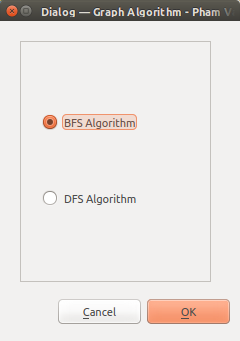
\includegraphics[scale=0.5]{images/pic4.png}
  \caption{Dialog lựa chọn thuật toán}
\end{figure}

Khung chương trình cho phép người dùng lựa chọn các thao tác:
\begin{description}
\item[Select] Lựa chọn đỉnh để kéo thả vào các vị trí thích hợp. Đỉnh được lựa chọn sẽ có dấu màu đỏ.
\item[Draw Vertex] Vẽ đỉnh trên màn hình. Nhãn của đỉnh được đánh số, tự động tăng khi có một đỉnh được tạo ra. Đỉnh được tạo ra tại vị trí con trỏ chuột, đỉnh sau khi tạo ra có thể \textbf{select} để chuyển đi vị trí mới.
\item[Draw Edge] Vẽ cạnh giữa hai đỉnh. Cạnh tự thay đổi theo vị trí của đỉnh.
\item[Play Animation] Chạy chương trình. Với mỗi bước của thuật toán, trạng thái các đỉnh, cạnh trên màn hình sẽ thay đổi. Cụ thể, đối với đỉnh, màu vàng nghĩa là chưa được duyệt, màu xanh là đã được thăm nhưng chưa hoàn thành, và màu xám là đã hoàn thành quá trình thăm. Với cạnh, các cạnh trong cây sẽ được tô màu xanh, lần lượt theo từng bước của thuật toán.
\end{description}
\begin{figure}[h!]
  \centering
  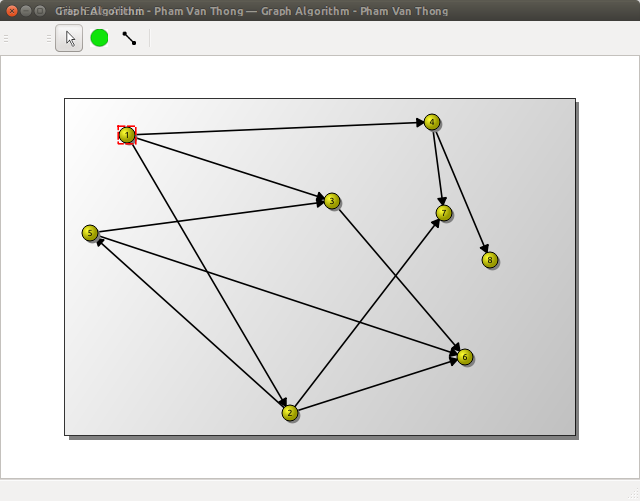
\includegraphics[scale=0.5]{images/pic5.png}
  \caption{Cửa sổ chính chương trình }
\end{figure}

\subsection{Tổng quan về chương trình}
Chương trình được lập trình trên C++, dựa trên bộ công cụ QT 5. Chương trình được chia thành các module nhỏ. Có 2 module chính:
\begin{description}
\item[Graphics Tool ] Thực hiện việc thiết kế giao diện dành cho quá trình mô phỏng, bao gồm việc nhập liệu cho người dùng như tạo đỉnh, cạnh, di chuyển đỉnh, và hiển thị các bước thay đổi của thuật toán. Bao gồm các class chính: \emph{GraphScene, GraphWidget, MainWindow, Dialog, Vertex, Edge}
\item[Algorithm] Thực hiện cài đặt mô hình thuật toán, lên kịch bảo cho quá trình mô phỏng. Bao gồm các class chính: \emph{Algorithm, DFSAnimation, BFSAnimation, Vertex, Edge}
\end{description}

Giữa hai module luôn có mối quan hệ khăng khít với nhau, một module nhận thông tin về các đối tượng đỉnh và cạnh được do người dùng nhập từ bàn phím chuyển tới cho module kia. Module còn lại tiếp nhận thông tin đó, và thực thi thuật toán, sau đó lên kịch bản để mô phỏng rồi chuyển tới cho module kia để trình diễn.

\subsection{Xây dựng các class chính}
\subsubsection{Class Vertex}
Class \emph{Vertex } mô phỏng đối tượng đỉnh, kế thừa từ lớp QGraphicsObject. Được cài đặt như sau:
\mnt{images/vertex.h}

Các thuộc tính và phương thức chính là:
\begin{description}
\item[Hàm tạo] Tạo đỉnh ở tọa độ là tham số được truyền vào. Xác định một số cờ hiệu và trạng thái mặc định của đỉnh.
\item[Các hàm thêm, xóa cung] Các hàm \textsf{addInEdge(), addOutEdge(), removeInEdge(), removeOutEdge()} thức hiện chức năng thêm, xóa các cung vào, ra tại đỉnh.
\item[Hàm inEdges(), outEdges()] Trả về danh sách cạnh tới đỉnh và ra khỏi đỉnh.
\item[Hàm boundingRect()] Định nghĩa lại phương thức ảo từ lớp QGraphicsObject, xác định phạm vi của đối tượng trong QGraphicsScene. Ví dụ nó giúp phát hiện được người dùng có đang trỏ chuột vào đối tượng không.
\item[Hàm paint()] Định nghĩa lại phương thức ảo từ lớp QGraphicsObject, xác định cách mà đỉnh đó được vẽ ra trên QGraphicsScene.
\item[Thuộc tính lớp interconnect] Xác định số thành phần liên thông của đồ thị.
\item[Thuộc tính m\_associate] Xác định đỉnh thuộc thành phần liên thông nào, giữ luôn vai trò đánh dấu trong các thuật toán BFS và DFS.
\item[Các hàm mouseEvent()] Vẽ lại đối tượng khi có thay đổi trên đối tượng.
\item[Các hàm và thuộc tính khác]
\end{description}

\subsubsection{Class Edge}
Class \emph{Edge} mô phỏng đối tượng cạnh, được kế thừa từ lớp QGraphicsObject. Cài đặt như sau:
\mnt{images/edge.h} 
Các phương thức và thuộc tính chính là:
\begin{description}
\item[Hàm tạo] Khởi tạo cạnh từ đỉnh nguồn tới đỉnh đích. Đặt trạng thái mặt định, thêm thông tin về cạnh tới, cạnh ra khỏi đỉnh vào đỉnh nguồn và đỉnh đích tương ứng.
\item[Hàm setSTate()] Thay đổi trạng thái của cạnh (Init, Inpath, ...)
\item[Hàm adjust()] Thay đổi cạnh để phù hợp với hiển thị (cạnh nối từ viền của đỉnh chứ không phải từ tâm của đỉnh, nếu hai đỉnh quá sát nhau thì không vẽ cạnh ra).
\item[Các hàm boundingRect(), paint()] Tương tự đối với class \emph{Vertex}.
\end{description}

\subsubsection{Class Algorithm}
Class \emph{Algorithm} được xây dựng như sau:
\mnt{images/algorithm.h}

Trong đó, các phương thức và thuộc tính chính là:
\begin{description}
\item[Hàm tạo ] Tạo action và \emph{Play Toolbar} dùng để chạy thuật toán, cài đặt các tham số khác như đỉnh nguồn mặc định, đỉnh đích mặc định (cho các thuật toán khác sẽ được phát triển tiếp), thời gian delay animation, ...
\item[Hàm getAlgorithm()] Khởi động hàm với thuật toán tương ứng \emph{BFS, DFS}
\item[Hàm newEdge()] Tạo cạnh mới, là phương thức ảo. Mỗi lớp con sẽ định nghĩa phương thức này khác nhau.
\item[Hàm resetState()] Khởi động lại trạng thái các đỉnh, cạnh sau mỗi lần duyệt xong (hủy đánh dấu, thay đổi màu sắc).
\item[Thuộc tính vertexList] Chứa danh sách các đỉnh, có thể xem dùng như danh sách kề (vì mỗi đỉnh chứa các danh sách outEdges và inEdges).
\item[Hàm generateAnimationList()] Phương thức ảo, mỗi lớp con sẽ định nghĩa phương thức này để trình diễn animation tương ứng của thuật toan ra màn hình.
\item[Hàm play()]  Được kết nối với action Play dùng để khởi động animation.
\item[Các thuộc tính và phương thức khác] Thực hiện các chức năng khác hoặc nhằm mục đích phát triển tiếp của chương trình.
\end{description}


\subsubsection{Class DFSAnimation, BFSAnimation}

Hai class này được cài đặt tương tự nhau, class BFSAnimation được cài đặt như sau:
\mnt{images/bfs.h}

Các phương thức và thuộc tính chính:
\begin{description}
\item[Hàm tạo] Kế thừa từ lớp Algorithm 
\item[Hàm newEdge()] Định nghĩa lại phương thức ảo từ lớp Algorithm.
\item[Hàm BFSVertex()] Thực hiện BFS tại 1 đỉnh.
\item[Hàm generateAnimationList()] BFS trên toàn bộ đồ thị, tạo animation.
\item[Thuộc tính animationGroup] Lưu animation sẽ được trình diễn.
\end{description}

Lớp DFSAnimation được cài đặt hoàn toàn tương tự.


\emph{Trong các class trên có dư thừa nhiều phương thức và thuộc tính để nhằm mục đích phát triển cho các thuật toán sau này.}

\subsection{Kết quả chạy thử}
Hình ảnh kết quả chạy thử chương trình:
\begin{figure}[h!]
  \centering
  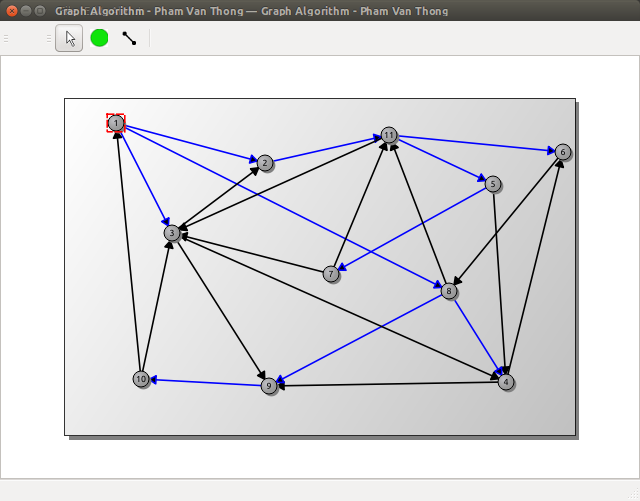
\includegraphics[scale=0.5]{images/pic6.png}
  \caption{Kết quả chạy thử BFS Animation}
\end{figure}

\begin{figure}[h!]
  \centering
  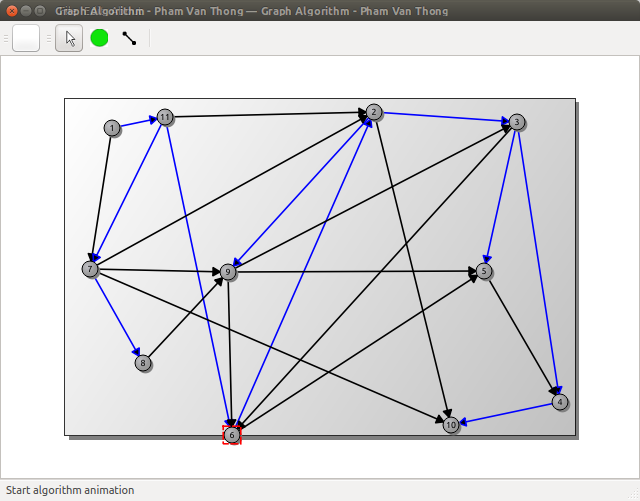
\includegraphics[scale=0.5]{images/pic7.png}
  \caption{Kết quả chạy thử DFS Animation}
\end{figure}

\newpage
\section{Thuật toán Bellman-Ford và thuật toán Dijkstra}
\subsection{Cài đặt}
Chương trình này chỉ thực hiện trên giao diện dòng lệnh, chia thành 3 class chính: Graph, Dijkstra, BellmanFord. Class Graph mô tả đối tượng đồ thị, lưu trữ thông tin về số đỉnh, ma trận trọng số của đồ thị, và các phương thức tạo nhập thông tin đồ thị từ file, hiển thị thông tin của đồ thị. Hai class còn lại thừa kế từ lớp Graph và mỗi lớp con thực hiện một thuật toán tương ứng.

Cài đặt cụ thể như sau:
\begin{figure}[h!]
  \centering
  \mnt{images/graph.h}
  \caption{graph.h}
\end{figure}


\begin{figure}[h!]
  \centering
  \mnt{images/graph.cc}
  \caption{graph.cc}
\end{figure}

\begin{figure}[h!]
  \centering
  \mnt{images/dijkstra.h}
  \caption{dijkstra.h}
\end{figure}

\begin{figure}[h!]
  \centering
  \mnt{images/dijkstra.cc}
  \caption{dijkstra.cc}
\end{figure}

\begin{figure}[h!]
  \centering
  \mnt{images/bellmanford.h}
  \caption{bellmanford.h}
\end{figure}

\begin{figure}[h!]
  \centering
  \mnt{images/bellmanford.cc}
  \caption{bellmanford.cc}
\end{figure}

\begin{figure}[h!]
  \centering
  \mnt{images/main.cc}
  \caption{main.cc}
\end{figure}


\subsubsection{Kết quả chạy thử}
Với ma trận kề như tương ứng thì kết quả tìm đường đi ngắn nhất với mỗi thuật toán như sau:
\begin{figure}[h!]
  \centering
  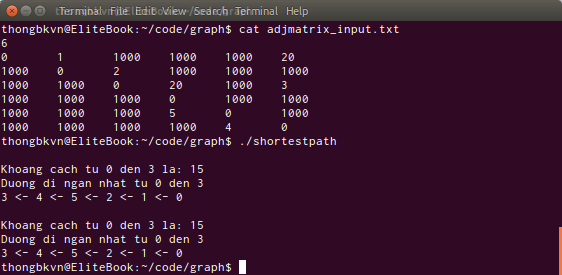
\includegraphics[scale=0.5]{images/pic8.png}
  \caption{Kết quả chạy thử chương trình tìm đường đi ngắn nhất}
\end{figure}

\section{Thuật toán cây khung nhỏ nhất}
Các thuật toán Kruskal và Prim được cài đặt như sau:
\begin{figure}[h!]
  \centering
  \mnt{images/prim.cc}
  \caption{Cài đặt thuật toán Prim}
\end{figure}

\begin{figure}[h!]
  \centering
  \mnt{images/kruskal.cc}
  \caption{Cài đặt thuật toán Kruskal }
\end{figure}
\paragraph{Kết quả chạy thử}
Với đồ thị đầu vào như sau:
\begin{figure}[h!]
  \centering
  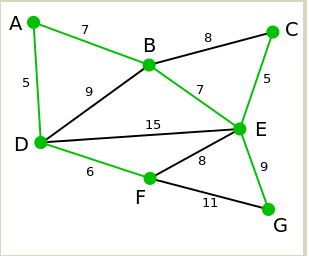
\includegraphics[scale=0.5]{images/pic9.png}
  \caption{Đồ thị đầu vào và kết quả mẫu}
\end{figure}

Kết quả thu được như sau:
\begin{figure}[h!]
  \centering
  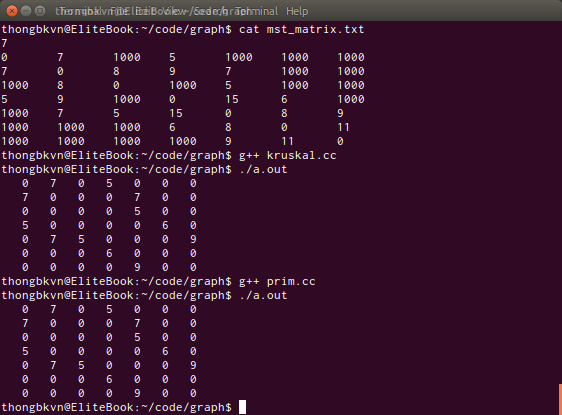
\includegraphics[scale=0.5]{images/pic10.png}
  \caption{Kết quả thu được với mỗi thuật toán}
\end{figure}


\section{Kết luận}
\subsection{Những kết quả đạt được}
\begin{itemize}
\item Những kiến thức tổng quan, cơ bản về đồ thị và một số thuật toán quan trọng trên đồ thị.
\item Xây dựng chương trình mô phỏng thuật toán DFS và BFS trên giao diện đồ họa.
\item Cài đặt các thuật toán tìm dường đi ngắn nhất trên đồ thị: Bellman-Ford và Dijkstra.
\item Cài đặt các thuật toán tìm cây khung nhỏ nhất của đồ thị: Prim và Kruskal.
\end{itemize}
\subsection{Hạn chế}
\begin{itemize}
\item Chương trình mô phỏng còn rất đơn giản, ít chức năng.
\item Chưa xây dựng được nhiều thuật toán trên giao diện đồ họa
\end{itemize}





\end{document}

